\documentclass[a4paper,12pt]{article} 

%%% Работа с русским языком
\usepackage{cmap}					% поиск в PDF
\usepackage{mathtext} 				% русские буквы в фомулах
\usepackage[T2A]{fontenc}			% кодировка
\usepackage[utf8]{inputenc}			% кодировка исходного текста
\usepackage[english,russian]{babel}	% локализация и переносы

%%% Дополнительная работа с математикой
\usepackage{amsmath,amsfonts,amssymb,amsthm,mathtools, gensymb} % AMS
\usepackage{icomma} % "Умная" запятая: $0,2$    ф--- число, $0, 2$ --- перечисление

%%Таблица
\usepackage[table,xcdraw]{xcolor}
\usepackage{caption}
\usepackage{floatrow}
\floatsetup[table]{capposition=top}
\floatsetup[wrapfigure]{capposition=bottom}
\usepackage{multirow}

%Отступы и поля 
\textwidth=18cm
\oddsidemargin=-1cm
\topmargin=-2cm
\textheight=25cm


%% Номера формул
\mathtoolsset{showonlyrefs=true} % Показывать номера только у тех формул, на которые есть \eqref{} в тексте.

%% Шрифты
\usepackage{euscript}	 % Шрифт Евклид
\usepackage{mathrsfs} % Красивый матшрифт

%% Свои команды
\DeclareMathOperator{\sgn}{\mathop{sgn}}

%% Перенос знаков в формулах (по Львовскому)
\newcommand*{\hm}[1]{#1\nobreak\discretionary{}
{\hbox{$\mathsurround=0pt #1$}}{}}

%% Стиль страницы
\usepackage{fancyhdr}

%% Для рисунков
\usepackage{graphicx}
\usepackage[export]{adjustbox}
\usepackage{float}
\usepackage{ragged2e}
\usepackage{wrapfig}

\pagestyle{fancy}
\begin{document}
\begin{titlepage}
\begin{center}
%\vspace*{1cm}
\large{\small ФЕДЕРАЛЬНОЕ ГОСУДАРСТВЕННОЕ АВТОНОМНОЕ ОБРАЗОВАТЕЛЬНОЕ\\ УЧРЕЖДЕНИЕ ВЫСШЕГО ОБРАЗОВАНИЯ \\ МОСКОВСКИЙ ФИЗИКО-ТЕХНИЧЕСКИЙ ИНСТИТУТ\\ (НАЦИОНАЛЬНЫЙ ИССЛЕДОВАТЕЛЬСКИЙ УНИВЕРСИТЕТ)\\ ФАКУЛЬТЕТ АЭРОКОСМИЧЕСКИХ ТЕХНОЛОГИЙ}
\vfill
\line(1,0){490}\\[1mm]
\huge{Лабораторная работа 4.3.2A}\\
\huge\textbf{Дифракция света на ультразвуковой волне в жидкости. \\
            A. Установка с вертикальной щелью}\\
\line(1,0){490}\\[1mm]
\vfill
\begin{flushright}
\normalsize{Рогозин Владимир}\\
\normalsize{\textbf{Группа Б03-106}}\\
\end{flushright}
\end{center}
\end{titlepage}
\fancyhead[L] {Работа 4.3.2A}

\textbf{Цель работы}:
изучение дифракции света на синусоидальной акустической решётке и наблюдение фазовой решётки методом тёмного поля.

\textbf{Оборудование}:
оптическая скамья, осветитель, два длиннофокусных объектива, кювета с жидкостью, кварцевый излучатель с микрометрическим винтом, генератор ультразвуковой частоты, линза, вертикальная нить на рейтере, микроскоп.

\section{Теоретические сведения}
В работе изучается дифракция света на фазовой решётке. Фазовая решётка создаётся в жидкости ультразвуковыми волнами и наблюдается методом тёмного поля.

\begin{wrapfigure}[15]{l}{0.4\textwidth}\label{fig: Diffraction on acoustic waves}
    \begin{center}
    \vspace{-20pt}
         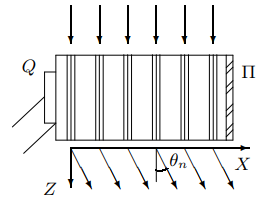
\includegraphics[width = 0.9\textwidth]{Diffraction on acoustic waves.png}
    \end{center}
    \caption{Дифракция световых волн на акустической решётке}
\end{wrapfigure}
При прохождении ультразвуковой (УЗ) волны через жидкость в ней возникают периодические оптические неоднородности, обусловленные разницей значений коэффициента преломления в областях сжатия и разрежения. Эти периодические неоднородности играют роль своеобразной дифракционной решётки для проходящего сквозь жидкость света.

В направлении оси $Z$ сквозь жидкость проходит световая волна, испытывающая дифракцию на акустической решётке. Поскольку скорость света значительно больше скорости звука, акустическую решётку можно считать неподвижной. Вызванное ультразвуком возмущение показателя преломления жидкости в нашем случае очень мало. При этом акустическую решётку можно рассматривать как тонкий фазовый экран.

При небольших амплитудах звуковой волны показатель преломления жидкости $n$ меняется по закону
\begin{equation}\label{eq: n(x)}
    n = n_0(1 + m\cos\Omega x),
\end{equation}
где $\Omega$ -- волновое число для УЗ-волны ($\Omega = 2\pi / \Lambda$ ), $\Lambda$ -- длина УЗ-волны, $m$ -- глубина модуляции показателя преломления, определяемая интенсивностью ультразвуковой волны $(m \ll 1)$.

Пусть фаза световых колебаний на передней поверхности жидкости равна нулю. Тогда на задней поверхности (т.е. в плоскости $z = 0$) она
равна
\begin{equation}\label{eq: delta_phi(x)}
    \varphi = k n L = \varphi_0(1 + m\cos\Omega x),
\end{equation}
где $L$ -- толщина слоя жидкости в кювете, $k$ -- волновое число для света, $\lambda$ -- длина световой волны, $\varphi_0 = k n_0 L$. Таким образом,
в плоскости $z = 0$ фаза световых колебаний является периодической функцией координаты $x$, иными словами -- УЗ-волна в жидкости создаёт фазовую дифракционную решётку.

Можно сформулировать качественный критерий, при выполнении которого можно считать акустическую решётку чисто фазовой, т.е. рассматривать её как тонкий фазовый экран. Для нашей задачи условие тонкого транспаранта можно записать в виде
\begin{equation}\label{eq: thin transarent condition}
    m \ll \frac{\Lambda}{L} \sqrt{\frac{\lambda}{\Lambda}}.
\end{equation}

Таким образом, чисто фазовая акустическая решётка реализуется лишь на достаточно слабой УЗ-волне. При повышении мощности ультразвука акустическая волна начинает работать как сложная амплитуднофазовая решётка.

В общем случае после прохождения через кювету световое поле представляет
совокупность не трёх, а большого числа плоских волн, распространяющихся под углами, определяемыми условием
\begin{equation}\label{eq: max condition}
    \Lambda \sin\theta_m = m\lambda \quad (m = 0, \pm 1, \text{ ...}).
\end{equation}
Каждая из этих волн соответствует одному из максимумов в дифракционной картине Фраунгофера.

Определяя на опыте положение дифракционных максимумов различного порядка, можно по формуле \eqref{eq: max condition} найти длину $\Lambda$ УЗ-волны и
вычислить скорость $v$ распространения ультразвуковых волн в жидкости, если известна частота $\nu$ колебаний кварцевого излучателя:
\begin{equation}\label{eq: wave's velocity}
    v = \Lambda\nu.
\end{equation}

\section{Экспериментальная установка}
Источник света $Л$ через светофильтр $Ф$ и конденсор $К$ освещает щель $S$, которая расположена в фокусе объектива $О_1$. 
\begin{figure}[H]\label{fig: Exp setup 1}
    \centering
    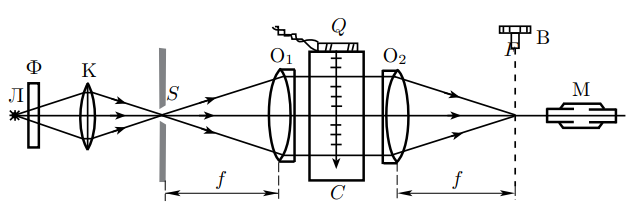
\includegraphics[width = 0.9\textwidth]{Exp setup 1.png}
    \caption{Схема наблюдения дифракции на акустической решётке}
\end{figure}
Выходящий из объектива параллельный пучок света проходит через кювету $C$ перпендикулярно направлению распространения УЗ-волн. Эти волны возбуждаются в жидкости пьезокварцевой пластинкой $Q$, прикреплённой к стенке кюветы. На кварцевую пластинку подаётся напряжение ультразвуковой частоты от генератора. В фокальной плоскости второго объектива $О_2$ образуется дифракционная картина, наблюдаемая при помощи микроскопа $М$. При этом обязательно применяют монохроматическое излучение (красный светофильтр).

Длина $\Lambda$ ультразвуковой волны определяется с помощью \eqref{eq: max condition}; в силу малости углов $\theta_m$ окончательное выражение может быть представлено в виде
\begin{equation}\label{eq: distance between max}
    l_m = mf\frac{\lambda}{\Lambda},
\end{equation}
где $l_m$ -- измеренное на опыте линейное расстояние между $m-$м и нулевым максимумами, а $f$ -- фокусное расстояние объектива $О_2$.

\subsection{Наблюдение оптических неоднородностей, создаваемых ультразвуковыми волнами в жидкости, методом тёмного поля.}
Попробуем теперь получить видимое изображение фазовой акустической решётки. Для этого, прежде всего, необходимо получить в поле зрения микроскопа изображение задней плоскости (считая походу световых лучей) кюветы. Это достигается с помощью вспомогательной положительной линзы $О$, которую располагают на оптической скамье за фокальной плоскостью объектива $О_2$ (рис. 3).
\begin{figure}[H]\label{fig: Exp setup 2}
    \centering
    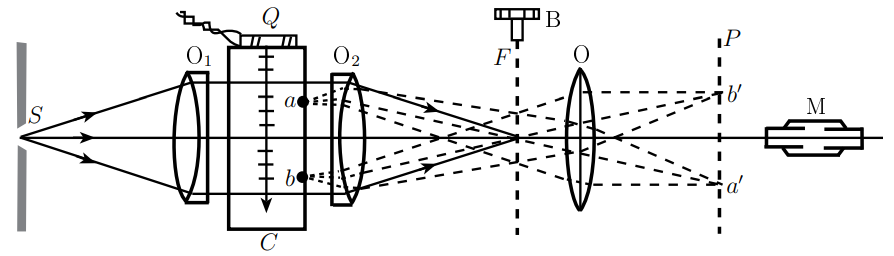
\includegraphics[width = 0.9\textwidth]{Exp setup 2.png}
    \caption{Наблюдение акустической решётки методом тёмного поля}
\end{figure}

Для наблюдения пространственной структуры фазовой решётки можно использовать метод \textit{тёмного поля}, основанный на устранении центрального дифракционного максимума с помощью специального экрана. В поле зрения микроскопа будут наблюдаться чередующиеся светлые и тёмные полосы, причём расстояние между тёмными полосами соответствует смещению в плоскости кюветы на $\Lambda / 2$. Таким образом, должно наблюдаться характерное для метода тёмного поля удвоение числа деталей рассматриваемой структуры.

\section{Обработка данных}
Все измерения проводились в красном свете $\lambda = (640 \pm 20)$ нм.
\subsection{Определение скорости ультразвука по дифракционной картине}
\begin{enumerate}
    \item 
    Соберём схему установки согласно рис. 2.
    \item 
    Найдём чёткую дифракционную картину и, перемещая излучатель с помощью микрометрического винта, оценим по порядку величины длину УЗ-волны как удвоенное расстояние между наиболее чёткими дифракционными картинами на одной частоте.
    \[\nu = 1,15 \text{ МГц}\]
    \[x_1 = 4,34 \text{ дел.} \quad x_2 = 5,01 \text{ дел.}\]
    Цена деления $\Delta = 1$ мм, погрешность измерений $\sigma = 0,05$ мм.
    В таком случае длина волны УЗ-волны будет равна удвоенному расстоянию между наиболее чёткими дифракционными картинами.
    \item 
    С помощью формулы \eqref{eq: wave's velocity} рассчитаем скорость звука в воде.
    \begin{equation}
        v = (1541 \pm 57) \text{ м/c}, \quad \varepsilon_v = 3,73 \%.
    \end{equation}
    \item 
    Далее, будем измерять положения $x_m$ дифракционных максимумов на различных частотах. Результаты измерений приведены в таблице ниже.
    \begin{table}[H]\label{tab: x_m different freq}
        \centering
        \begin{tabular}{|
            >{\columncolor[HTML]{FFFFFF}}c |
            >{\columncolor[HTML]{FFFFFF}}c |
            >{\columncolor[HTML]{FFFFFF}}c |
            >{\columncolor[HTML]{FFFFFF}}c |}
            \hline
            {\color[HTML]{000000} $\nu$, МГц} & {\color[HTML]{000000} 1,149} & {\color[HTML]{000000} 3,46}  & {\color[HTML]{000000} 6,09}  \\ \hline
            {\color[HTML]{000000} Порядок максимума} & {\color[HTML]{000000} $x_m$, дел.} & {\color[HTML]{000000} $x_m$, дел.} & {\color[HTML]{000000} $x_m$, дел.} \\ \hline
            {\color[HTML]{000000} 2}         & {\color[HTML]{000000} 16,90} & {\color[HTML]{000000} 14,05} & {\color[HTML]{000000} 12,25} \\ \hline
            {\color[HTML]{000000} 1}         & {\color[HTML]{000000} 16,55} & {\color[HTML]{000000} 15,10} & {\color[HTML]{000000} 14,20} \\ \hline
            {\color[HTML]{000000} 0}          & {\color[HTML]{000000} 16,20} & {\color[HTML]{000000} 16,20} & {\color[HTML]{000000} 16,20} \\ \hline
            {\color[HTML]{000000} -1}          & {\color[HTML]{000000} 15,89} & {\color[HTML]{000000} 17,28} & {\color[HTML]{000000} 18,20} \\ \hline
            {\color[HTML]{000000} -2}          & {\color[HTML]{000000} 15,50} & {\color[HTML]{000000} 18,40} & {\color[HTML]{000000} 20,22} \\ \hline
        \end{tabular}
        \caption{Данные измерений координат максимумов}
    \end{table}
    Цена деления $\Delta = 0,4$ мм, погрешность измерений $\sigma = 0,1$ мм.
    По данным из таблицы потсроим график зависимости координаты максимума от его порядка.
    \item 
    Запишем фокусное расстояние линзы $F = 30$ см. После этого найдём угол наклона прямой для каждой из частот и, используя формулу \eqref{eq: distance between max}, вычислим длину волны $\Lambda$. Затем по формуле \eqref{eq: wave's velocity} найдём скорость звука в воде.
    \begin{table}[H]\label{tab: wave velocity results}
        \centering
        \begin{tabular}{|
            >{\columncolor[HTML]{FFFFFF}}c |
            >{\columncolor[HTML]{FFFFFF}}c |
            >{\columncolor[HTML]{FFFFFF}}c |
            >{\columncolor[HTML]{FFFFFF}}c |}
            \hline
            {\color[HTML]{000000} $\nu$, МГц}     & {\color[HTML]{000000} 1,149}         & {\color[HTML]{000000} 3,46}         & {\color[HTML]{000000} 6,09}        \\ \hline
            {\color[HTML]{000000} $\Lambda$, мкм} & {\color[HTML]{000000} $1390 \pm 48$} & {\color[HTML]{000000} $440 \pm 14$} & {\color[HTML]{000000} $240 \pm 8$} \\ \hline
            {\color[HTML]{000000} $v$, м/с} &
              {\color[HTML]{000000} $1598,61 \pm 55,76$} &
              {\color[HTML]{000000} $1527,17 \pm 47,80$} &
              {\color[HTML]{000000} $1465,26 \pm 45,86$} \\ \hline
            {\color[HTML]{000000} $\varepsilon$, $\%$} &
              {\color[HTML]{000000} 3,48} &
              \cellcolor[HTML]{FFFFFF}{\color[HTML]{000000} 3,13} &
              \cellcolor[HTML]{FFFFFF}{\color[HTML]{000000} 3,13} \\ \hline
        \end{tabular}
        \caption{Результаты вычисления скорости звука в воде}
    \end{table}
    \item 
    Сравним полученные значения с табличным: $v_{табл.} \approx 1500$ м/c. Все значения кроме одного совпадают в пределах погрешности с табличным.
\end{enumerate}

\subsection{Определение скорости ультразвука методом тёмного поля}
\begin{enumerate}
    \item 
    Соберём установку как на рис. 3.
    \item 
    Для различных значений частот генератора измерим количество тёмных полос и расстояние между крайними минимумами. По формуле $\Lambda = 2 \Delta / N \cdot x$, где $x = 70$ мкм -- цена деления шкалы микроскопа, $N$-- количество видимых тёмных (светлых) полос, найдем длину волны для различных частот, отсюда, по формуле \eqref{eq: wave's velocity}, найдем скорость звука в воде. Результаты представлены в таблице ниже.
    \begin{table}[H]\label{tab: wave velocity and length results}
        \centering
        \begin{tabular}{|
            >{\columncolor[HTML]{FFFFFF}}c |
            >{\columncolor[HTML]{FFFFFF}}c |
            >{\columncolor[HTML]{FFFFFF}}c |
            >{\columncolor[HTML]{FFFFFF}}c |
            >{\columncolor[HTML]{FFFFFF}}c |}
            \hline
            {\color[HTML]{000000} $\nu$, МГц} &
              {\color[HTML]{000000} $\Delta$, дел.} &
              {\color[HTML]{000000} $N$, штук} &
              {\color[HTML]{000000} $\Lambda$, мкм} &
              \cellcolor[HTML]{FFFFFF}{\color[HTML]{000000} $v$, м/c} \\ \hline
            {\color[HTML]{000000} 1,154} & {\color[HTML]{000000} 70} & {\color[HTML]{000000} 8}  & {\color[HTML]{000000} $1400 \pm 20$} & {\color[HTML]{000000} $1615,6 \pm 23,1$} \\ \hline
            {\color[HTML]{000000} 1,52}  & {\color[HTML]{000000} 74} & {\color[HTML]{000000} 10} & {\color[HTML]{000000} $1120 \pm 20$} & {\color[HTML]{000000} $1702,4 \pm 23,0$} \\ \hline
            {\color[HTML]{000000} 1,816} & {\color[HTML]{000000} 80} & {\color[HTML]{000000} 14} & {\color[HTML]{000000} $840 \pm 11$}  & {\color[HTML]{000000} $1525,4 \pm 19,1$} \\ \hline
        \end{tabular}
        \caption{Длина волны и скорость звука на различных частотах}
    \end{table}
\end{enumerate}

\newpage
\section{Вывод}
В данной работе была изучена дифракция света на ультразвуковой волне в жидкости:

\begin{itemize}
    \item Трёмя способами была найдена скорость звука в воде, результаты в пределах погрешности совпали с табличным значением $v = 1500$ м/с.
    
    \item
   С помощью метода тёмного поля было получено изображения акустической решётки.
\end{itemize}

%%%%%%%%%%%%%%%%%%%%%%%%% Графики
\newpage
\begin{figure}[H]\label{fig: x_m(m)}
    \centering
    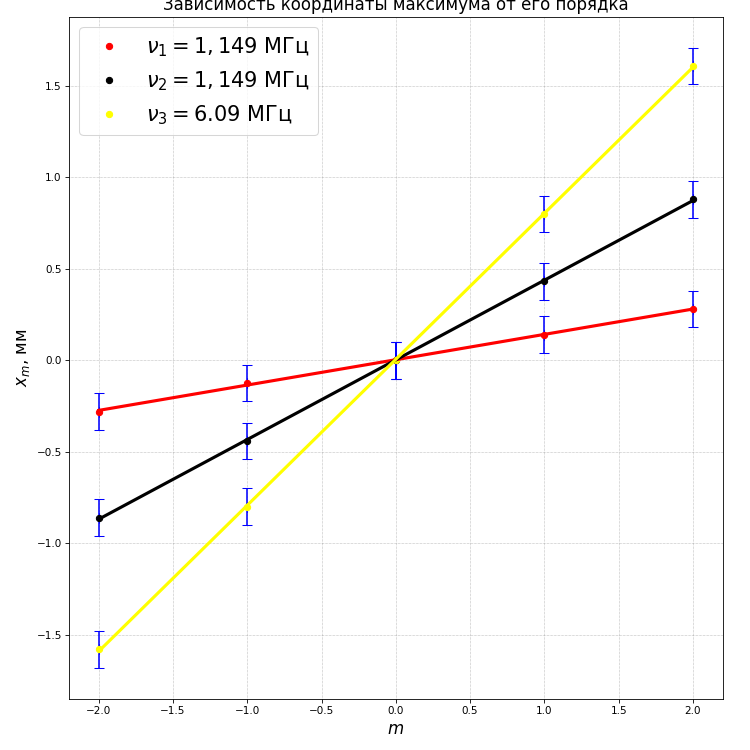
\includegraphics[width = 0.9\textwidth]{x_m(m).png}
\end{figure}
\[k_{\nu_1} = (1,38 \pm 0,02)\cdot 10^{-4} \text{ м}, \quad \varepsilon_k = 1,55 \%\]
\[k_{\nu_2} = (4,35 \pm 0,02)\cdot 10^{-4} \text{ м}, \quad \varepsilon_k = 0,5 \%\]
\[k_{\nu_3} = (7,98 \pm 0,03)\cdot 10^{-4} \text{ м}, \quad \varepsilon_k = 0,36 \%\]

%%%%%%%%%%%%%%%%%%%%%%%%%
\end{document}
